\chapter{基于人类偏好对齐的检索增强对话生成}
\section{引言}

垂直领域对话场景下的用户问题往往多样而复杂,模型难以从输入的用户问题中准确理解用户的真实意图,即在语义检索和回答生成过程中存在数据分布偏差,导致模型生成不符合用户预期的回答。如图\ref{alignment_problem_show_case}所示,对于描述不够清晰明确的垂直领域用户问题,知识库检索到的知识文档内容与用户意图存在偏差,这导致LLM生成的红色回答较为简略、不符合用户预期。若能对齐人类意图与模型理解,即可得到图中更详细和信息丰富的绿色回答。通过向人类偏好对齐,能够进一步提升垂直领域检索增强对话生成任务的用户交互体验,因此LLM的人类偏好对齐研究受到越来越多研究者的关注。

\begin{figure}[htbp]
	\centering
	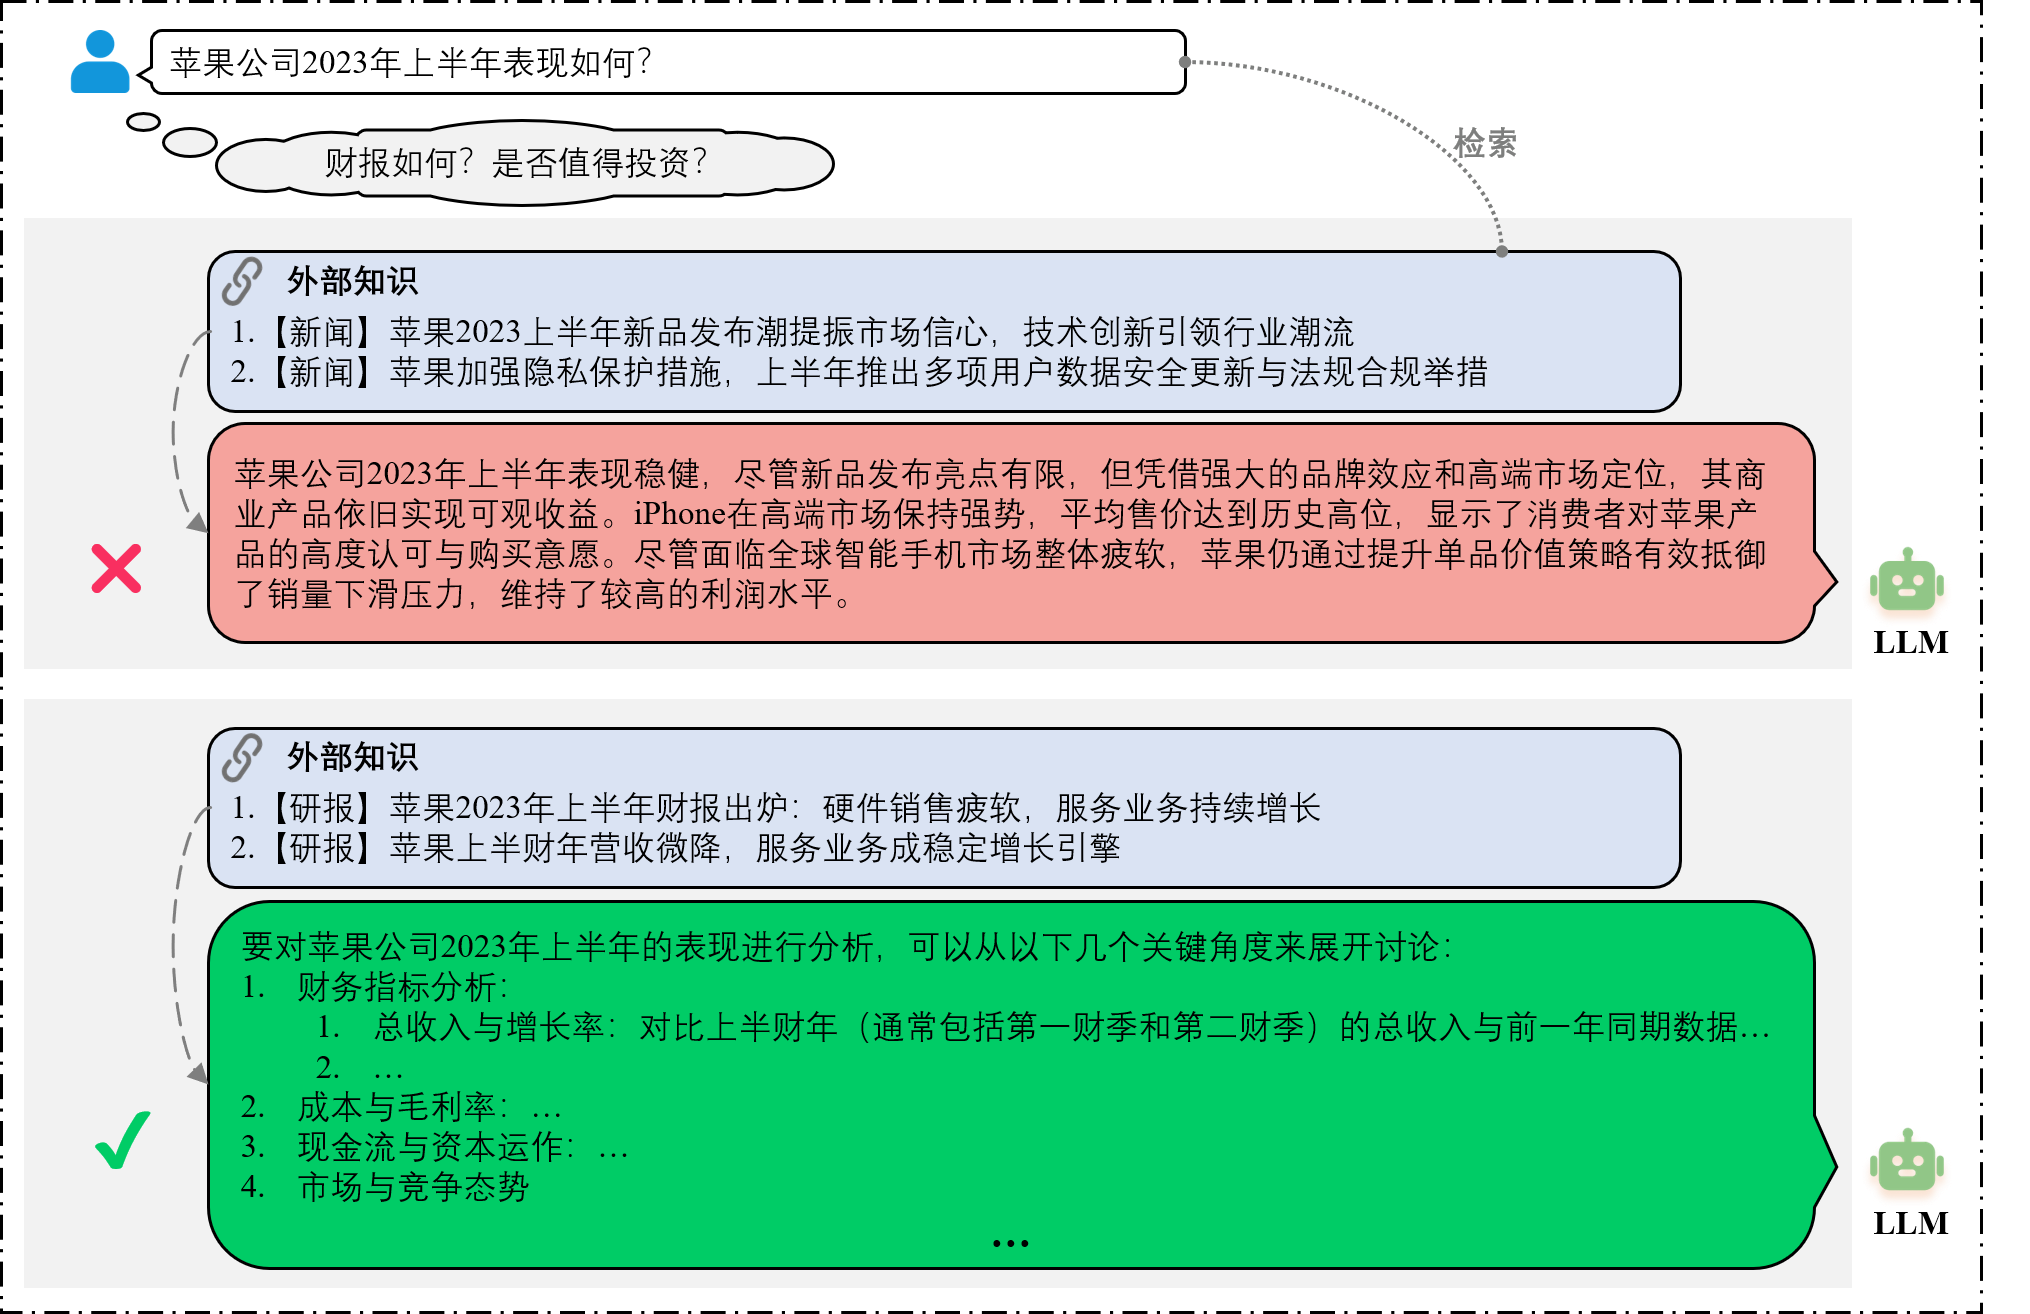
\includegraphics[scale=0.45]{Fig/alignment_problem_show_case.png}
	\caption{\label{alignment_problem_show_case}垂直领域对话场景下的模型理解偏差问题示例。}
\end{figure}

为了实现LLM的人类偏好对齐,Long等人\cite{DBLP:conf/nips/Ouyang0JAWMZASR22}提出了RLHF方法,首先采集高质量数据集对语言模型进行监督微调(SFT),再基于SFT模型的生成内容收集人类偏好排名数据集,并训练奖励模型(RM),最后执行PPO强化学习进一步微调SFT模型,显式地引入了人类偏好和主观意见,使得模型生成的内容更符合人类的偏好。然而,RLHF方法存在一定的局限性。一方面,RLHF需要大规模的人类偏好标注数据,垂直领域的训练数据则更加难以获取。另一方面,RLHF使用PPO强化学习来训练LLM,训练过程复杂且效果稳定性差。为了应对RLHF方法存在的问题,Rafailov等人\cite{DBLP:conf/nips/RafailovSMMEF23}提出DPO算法,通过引入SFT约束,在不降低性能的情况下提升训练的稳定性。Dong等人\cite{DBLP:journals/corr/abs-2304-06767}提出RAFT方法,无需使用强化学习,进一步提升稳定性和鲁棒性。Bai等人\cite{DBLP:journals/corr/abs-2212-08073}提出RLAIF方法,使用LLM代替人类完成偏好标注工作,一定程度上缓解了数据稀缺问题。然而,上述方法需要训练对话模型本身,随着大型语言模型的发展,对话模型尺寸也不断增大,且部分闭源模型只能通过API访问,因此基于训练的方法受到对话模型的尺寸和访问限制难以应用和迁移。

与训练模型使之对齐人类意图不同,Cheng等人\cite{DBLP:journals/corr/abs-2311-04155}提出BPO算法,使用户问题中的用户意图对齐模型理解。然而,BPO算法存在一些局限性。一方面,BPO利用LLM直接对用户问题进行优化,在检索增强应用场景下,没有考虑检索到的知识文档信息,存在性能瓶颈。另一方面,BPO使用LLM进行用户问题优化,所生成的内容可能受到LLM的幻觉问题影响,因此数据有效性不足。

针对上述问题,本文提出一种基于人类偏好对齐的检索增强对话生成方法,通过采集人类对检索增强对话的偏好反馈数据,利用LLM分别针对数据库检索和对话生成进行优化,各自得到一个新的用户问题,基于优化后的问题,再次进行相关文档块检索和对话生成,根据生成的回答内容进行样本有效性验证,并用有效样本构建三元组训练数据集,训练一个单独Seq2Seq模型作为问题优化器,在推理时自动将用户意图对齐模型理解,实现与模型无关的、稳定的人类偏好对齐。

% 对于用户问题“苹果公司2023年上半年表现如何?”,在金融领域,这通常表示用户关注苹果公司在2023年上半财年的财务和市场表现。然而,将用户问题直接用于检索增强生成,得到图中红色的回答,由于知识库中的语义检索模型在通用语料上训练,不具有垂直领域相关的知识,因此检索到的外部知识均为苹果产品相关的新闻,没有财务数据,这导致LLM的回答范围受限于苹果新产品和新技术,而没有从财务角度进行分析,且回答较为简略、不够详细,不符合用户预期。若能将用户问题与语义检索模型和回答生成模型对齐,更符合用户意图的外部知识文档为苹果公司上半财年的财务数据和研究报告,基于这类数据,即可得到图中更详细和信息丰富的绿色回答,即符合用户预期的回答。预期回答不仅总结了苹果公司的财务表现和市场表现,还从多个角度全面而详细地进行了分析。

% 现有大部分人类偏好对齐方法主要通过训练对话模型,使其向人类偏好对齐,例如指令微调\cite{DBLP:conf/iclr/WeiBZGYLDDL22}方法、RLHF\cite{DBLP:conf/nips/Ouyang0JAWMZASR22,DBLP:journals/corr/abs-2212-08073}方法、RLAIF\cite{DBLP:journals/corr/abs-2212-08073}方法、DPO\cite{DBLP:conf/nips/RafailovSMMEF23}方法等等。然而,这类方法需要训练对话模型本身,随着大型语言模型的发展,对话模型尺寸也不断增大,且部分闭源模型只能通过API访问,因此基于训练的方法受到对话模型的尺寸和访问限制难以应用和迁移。

\section{问题定义}

给定垂直领域用户问题$Q$,外部知识库检索与此相关的文档序列$D = [d_1, \dots, d_k]$,对话系统需要基于$Q$和$D$输出符合用户偏好的问题回复$R$。此任务的主要挑战是需要对齐用户意图和模型理解,使得所生成的回复符合人类偏好。

\section{本章方法}

\subsection{方法总体方案}

\begin{figure}[htbp]
	\centering
	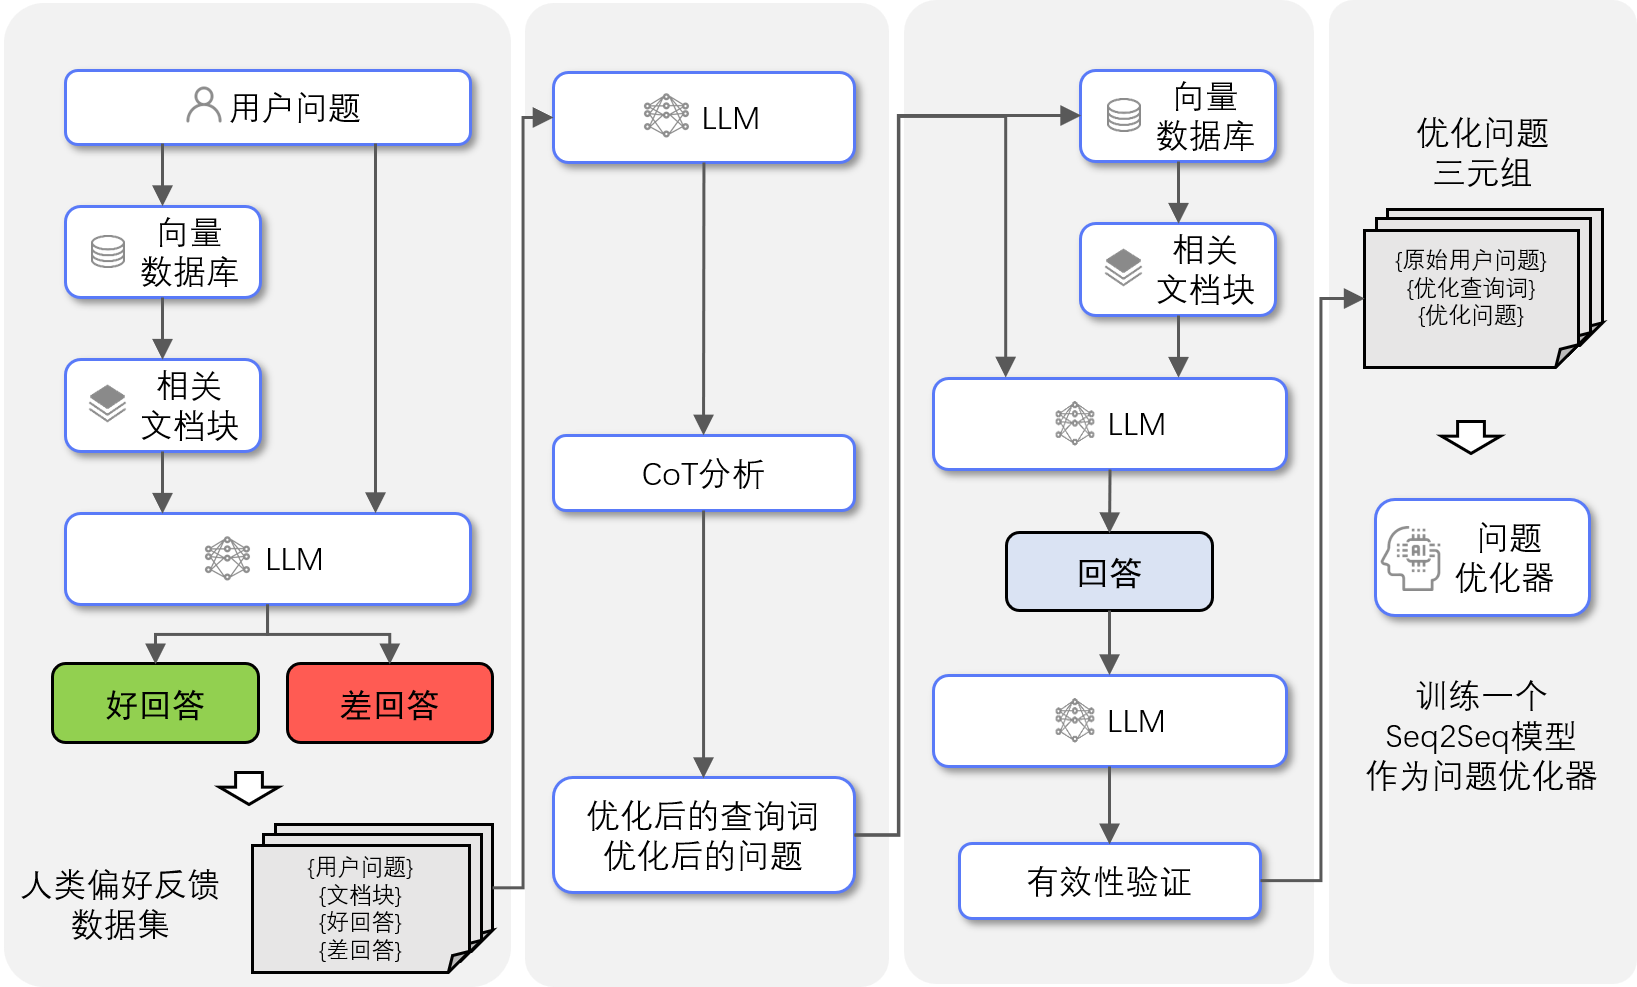
\includegraphics[scale=0.57]{Fig/qahf_framework.png}
	\caption{\label{qahf_framework}基于人类偏好对齐的检索增强对话生成框架图。}
\end{figure}

本章研究一种基于人类偏好对齐的检索增强对话生成的方法,该任务通常需要收集对话模型在各类真实场景下的对话,然后由人类完成偏好标注,最后通过PPO强化算法或其他算法训练对话模型,以达到偏好对齐的目的。而PPO强化学习在大型语言模型上非常具有挑战性,训练效果稳定性低。因此,本章提出基于人类反馈的问题对齐(Query Alignment with Human Feedback, QAHF),基于人类偏好反馈数据训练一个单独的问题优化器,避免直接训练对话模型,从而实现与模型无关的、非侵入的人类偏好对齐。如图\ref{qahf_framework}所示,QAHF方法主要包括四个阶段:1)人类偏好数据采集阶段;2)优化问题构建阶段;3)问题有效性验证阶段;4)问题优化器训练阶段。

\renewcommand{\algorithmcfname}{算法}
\begin{algorithm}
	\caption{基于人类偏好对齐的检索增强对话生成方法} %算法的名字
	% {\bf Input:} %算法的输入, \hspace*{0.02in}用来控制位置,同时利用 \\ 进行换行
	% Network and energy parameters $V^{vec},V^{c},\zeta^c,\zeta^{vec}$ etc; convergence tolerance $\epsilon$; iteration $\tau=1$ \\
	%	\hspace*{0.02in} {\bf Output:} %算法的结果输出
	
	\begin{algorithmic}[1]
		\STATE {\bf 输入:} %算法的输入, \hspace*{0.02in}用来控制位置,同时利用 \\ 进行换行
		用户问题集合$Q$,知识文档块集合$D$,对话模型$M$,问题优化器$\pi_\theta$.
		% \STATE {\bf Output:} $P_n^*,f_n^*,a_n^*$ %算法的结果输出
		\STATE {\bf for} q {\bf in} Q {\bf do}
		\STATE \qquad 从$D$中检索与$q$相关性Top-3的知识文档$\{d_1, d_2, d_3\}$
		\STATE \qquad 将$q$与$\{d_1, d_2, d_3\}$输入$M$,基于随机采样收集回答组$\{r_1, r_2, ...\}$
		\STATE \qquad 通过回答质量评测标准对$r_j$计算偏好一致性$c_j$
		\STATE \qquad 选择偏好一致性分数最高和最低的回答$r_{good}$和$r_{bad}$
		\STATE {\bf end for}
		\STATE {\bf for} 偏序数据对 i = 1, ..., N {\bf do}
		\STATE \qquad 通过模型$M$获取偏好特征思维链分析$A$
		\STATE \qquad 结合思维链分析$A$,获取优化后的检索问题$q^i_{search}$和优化后的用户问题$q^i_{qa}$
		\STATE \qquad 从$D$中检索与$q^i_{search}$相关性Top-3的知识文档$\{d^i_1, d^i_2, d^i_3\}$
		\STATE \qquad 将$q^i_{qa}$与$\{d^i_1, d^i_2, d^i_3\}$输入$M$,收集回答$r_i$
		\STATE \qquad 通过模型$M$计算优化问题有效性$c_i$
		\STATE \qquad {\bf if} $c_i > threshold$ {\bf do}
		\STATE \qquad \qquad 将$c_i$加入优化问题数据集$O$
		\STATE {\bf end for}
		\STATE 使用预训练模型参数初始化问题优化器的网络参数$\theta$
		\STATE {\bf while} 不收敛 {\bf do}
		\STATE \qquad 从优化问题数据集$O$中均匀采样三元组样本
		\STATE \qquad 通过公式(4-1)得到样本输出
		\STATE \qquad 通过AdamW优化算法更新$\theta$
		\STATE {\bf end while}
		% \STATE Initialize variable: $\forall a_n\in \mathbb{V}$, set $a_n=1$.
		% \STATE Obtain $P_n^*,f_n^*$ by solving $P2$ without considering $(C1)$.
		% \STATE Check $(C1)$ has been satisfied or not.
		% \STATE {\bf If} $(C1)$ has been satisfied:
		% \STATE \qquad put $P_n^*,f_n^*$ into $P3$
		% \STATE \qquad Obtain $a_n^*$ by solving $P3$.
		% \STATE \qquad \Return $P_n^*,f_n^*,a_n^*$.
		% \STATE {\bf Else}: 
        % \STATE \qquad Traversing all vehicles, find $n=\arg max(q_n)$
        % \STATE \qquad $K_n=K_n-\mathbb{K}$
        % \STATE \qquad Jump to the step 5
	\end{algorithmic}
\end{algorithm}

\subsection{人类偏好数据采集阶段}

为了将模型理解与人类偏好对齐,本节需要对垂直领域对话中的人类偏好进行建模,以提取人类偏好特征,用于后续的优化问题生成。语言模型的训练方式采用Next Token Prediction(NTP)任务,偏好对齐的目标是找到原始用户问题与真实用户意图的内在联系,从而对原始用户问题和反映真实意图的优化用户问题的条件概率分布进行建模,具体的数据采集步骤如下。

本节首先通过收集垂直领域开源数据集和爬取互联网媒体语料,构建了一个垂直领域问答数据集,该数据集样本为“问题-回答”对,数据样本的问答主题为垂直领域相关专业问题。然后,本章使用基于规则的方法,过滤掉数据集中的低质量样本,以保证样本的用户问题存在优化空间,具体做法是:1)先过滤筛除输入、输出长度低于10个标识符的过短样本;2)然后基于百科词条与开源数据集构建垂直领域专有名词词汇表,筛除样本中不包含专有名词的领域无关样本。本章主要关注单轮对话的对话生成。

随后,在向量数据库中检索与用户问题相关的文档块,并将结果输入LLM,通过随机采样的生成策略,从LLM的语言空间中采样得到多组不同的回答。最后,通过人工标注的方式,根据回答质量评判标准对LLM回答进行偏序关系标注,从每组回答中选出综合评分更高的回答作为“好回答”,评分最低的回答作为“差回答”,“好回答”与“坏回答”的Pairwise样本构成偏序回答对,其与原始用户问题和相关文档块共同组成人类偏好反馈数据集。该标注步骤引入人类的偏好信息,即回答评分和排名。其中,回答质量评判标准包含5个维度,即准确性、完整性、逻辑性、表达能力和有效建议,以确保标注标准的客观性和一致性,每个维度的评分取值范围为0、1、2分,分别表示“不符合预期”、“不太符合预期”和“较为符合预期”,最终通过加权平均计算得到样本的偏好一致性评分$C$。
\begin{equation}
	C = \frac{1}{5}\sum_{i=1}^{5}c_i
\end{equation}
其中,$c_i$分别表示不同维度的评分。

\subsection{优化问题构建阶段}

随后,本节通过利用LLM的基础推理能力,基于人类偏好反馈数据集中的偏序回答对,对原始用户问题进行优化。问题优化任务包含多个推理步骤,即首先从偏序回答对中提取出人类偏好特征,分析原始用户问题中包含的真实意图,并最终对原始用户问题进行重写,得到优化后的用户问题。问题优化任务属于复杂逻辑推理任务,且由于LLM采用自回归的文本生成方式,模型输出内容会受到前面单词的影响,因此直接基于偏序回答对进行问题优化,结果的不稳定性较大,导致进一步加剧LLM幻觉问题,无法有效完成人类偏好对齐。同时,由于检索增强对话输入包含多个外部知识文档块,问题优化任务的输入普遍具有较长的上下文,若使用Few-shot提示推理策略,模型输入将超过2048个标识符,导致模型推理出现外推问题,即推理长度超过模型训练长度后,模型推理的性能显著下降,具体表现为困惑度(Perplexity,PPL)等指标显著上升。
为解决上述问题,本节使用基于Zero-shot-CoT的提示工程方法进行用户问题优化,通过扩展LLM推理步骤,在改写用户问题前补充流畅而符合逻辑的上下文,利用LLM的内部参数知识引导模型自身完成人类偏好特征识别,从而改变其推理结构,最大化发挥LLM在问题优化任务上的性能。

在检索增强对话生成任务中,用户问题会分别被用于本地知识库的知识文档召回和LLM回答生成。知识文档召回计算用户问题和文档块之间的本文相似度与语义相似度,而LLM回答生成需要以用户问题为指令进行精准解答,这两个场景的任务目标存在差异,使用相同的用户问题分别进行文档召回和回答生成存在性能瓶颈。因此,本节分别针对本地知识库的知识文档召回和LLM回答生成场景各自生成一个优化问题,使得在新的用户问题下,检索增强对话系统生成的回答分布更趋近于“好回答”的分布,区别于“差回答”的分布。

本节所使用的问题优化提示词如表\ref{query_optimize_prompt}所示。当模型输出结果不符合提示词中的输出格式要求时,后处理过程中无法提取出有效的优化问题。对此,本节的解决方法是,在后处理抛出匹配异常时,调整模型推理超参数,即提高temperature和top\_p,使预测词概率被拉平,并再次进行模型推理,以此循环直到模型输出符合预期格式要求。

\begin{table}
	\caption{\label{query_optimize_prompt}问题优化提示词格式。}
	\centering{}%
	\small 
	\begin{tabular}{c}
		\toprule[2pt]
		问题优化提示词\tabularnewline
		\hline 
		\begin{tabular}{p{15cm}}
			\# SYSTEM\\你是一个大语言模型Prompt工程专家,你将根据我提供的信息完成我指定的任务。其中,QUERY表示用户输入的问题,DOCS是在数据库中检索得到的与QUERY相关的知识文档,GOOD RESPONSE是相比于BAD RESPONSE更符合人类偏好的LLM回复。 \\ \# QUERY \\ 作为个人知识答疑助手,请根据上述参考内容回答下面问题,答案中不允许包含编造内容。 \\ 问题是:<original query> \\ \# DOCS \\ <docs> \\ \# GOOD RESPONSE \\ <good response> \\ \# BAD RESPONSE \\ <bad response> \\ \# TASK \\ 你的任务是: \\ 1. 判断检索到的DOCS是否与QUERY相关,以及DOCS中的信息是否能够回答QUERY中的问题; \\ 2. 从事实性、完整性、逻辑性三个方面对比GOOD RESPONSE和BAD RESPONSE,分析可能导致LLM给出BAD RESPONSE的原因; \\ 3. 若DOCS与QUERY相关性不高,重写一个新的Query,用于数据库检索,使得检索到的DOCS的相关性更高,否则不需要重写; \\ 4. 作为专业的Prompt工程师,再重写一个新的QUERY,用于输入LLM,使得LLM更有可能给出GOOD RESPONSE。
		\end{tabular} \\
		\bottomrule[2pt]
	\end{tabular}
\end{table}

\subsection{问题有效性验证阶段}

LLM生成的优化问题可能仍然存在理解偏差问题,这类无效样本将成为数据集噪声,若直接使用带噪声的数据进行后续模型训练,可能会进一步加重模型理解偏差,反而损害模型性能。因此,有必要对上一步骤所生成的优化问题数据进行筛选过滤,剔除对人类偏好对齐产生负向优化的低质量样本。相较于直接对数据集样本中的优化问题进行有效性评估,引入问题优化后的模型回复能够更好地观察优化问题对文档召回和回答生成的影响,从而提升有效性评估的准确率。因此,本节将优化后的用户问题重新输入系统,进行知识文档召回后得到新的模型回复,并利用大型语言模型的Self-Criticism能力\cite{DBLP:conf/emnlp/TanSQQQXQ23},对新回复的质量进行评判,以筛选出有效的偏好数据样本,提高数据集信噪比,并得到最终的优化问题三元组数据集。与上一节相同,本节同样使用Zero-shot-CoT方法进行问题有效性验证,以提升LLM的准确性。

\begin{table}
	\caption{\label{query_validation_prompt}问题有效性验证提示词格式。}
	\centering{}%
	\small 
	\begin{tabular}{c}
		\toprule[2pt]
		有效性验证提示词\tabularnewline
		\hline 
		\begin{tabular}{p{15cm}}
			\#SYSTEM \\ 你是一个大语言模型Prompt工程专家,你将根据我提供的信息完成我指定的任务。其中,QUERY表示用户输入的问题,DOCS是在数据库中检索得到的与QUERY相关的知识文档,RESPONSE是LLM的回复。 \\ \# QUERY \\ 作为个人知识答疑助手,请根据上述参考内容回答下面问题,答案中不允许包含编造内容。 \\ 问题是:<original query> \\ \# DOCS \\ <docs> \\ \# RESPONSE \\ < response> \\ \# TASK \\ 你的任务是: \\ 1. 判断检索到的DOCS是否与QUERY相关,以及DOCS中的信息是否能够回答QUERY中的问题; \\ 2. 判断RESPONSE是否能够准确、可靠地回答QUERY; \\ 3. 对RESPONSE进行评分,分数取值范围为[1, 10]。 \\ 
		\end{tabular} \\
		\bottomrule[2pt]
	\end{tabular}
\end{table}

其中,本节所使用的问题有效性验证提示词如表\ref{query_validation_prompt}所示,有效性验证过程包含三个步骤:1)计算知识文档与用户问题的相关性,即验证优化后的问题是否与知识文档的语义空间完成对齐;2)计算模型回答的正确性,即验证优化后的问题与对话模型是否完成对齐;3)根据上述相关性和正确性结果,给出最终的问题优化有效性评分,取值范围为[1, 10]。提示词中对模型输出格式进行了约束,故本节采用正则表达式匹配的方式从模型输出中提取评分结果。

\subsection{问题优化器训练阶段}

基于前述步骤所构建的人类偏好数据集,训练一个Seq2Seq\cite{DBLP:journals/corr/abs-2309-16609}模型作为问题优化器,实现模型无关的、可插拔的用户问题自动优化。形式上,给定原始用户问题$Q_{ori}$,优化器生成优化后的用户问题$Q_{opt}$:
\begin{equation}
	Q_{opt} = [Q_{search}, [SEP], Q_{qa}]
\end{equation}
其中,$Q_{search}$表示用于数据库检索的问题,$Q_{qa}$表示用于回答生成的问题,$[SEP]$为特殊标识符,用于分隔$Q_{search}$和$Q_{qa}$。

本节使用交叉熵损失函数作为训练目标,损失函数定义为:
\begin{equation}
	\mathcal{L}=-\frac{1}{N} \sum_{t=1}^N \log P\left(x_t \mid Q_{\text{ori}}, x_{<t}\right)
\end{equation}
其中,$N$是$Q_{opt}$的长度,$x_t$表示$Q_{opt}$中的第$t$个标识符。本章选择Qwen-7B作为基座模型,以更好地学习$Q_{ori}$和$Q_{opt}$之间的隐式偏好映射。同时,在目前的主流LLM中,7B模型的参数量相对较小,能够以更低的成本进行训练和推理,具有更低的推理延迟,作为本方法中的问题优化器具有一定优势。

\section{实验结果}

\subsection{数据集介绍}

\begin{itemize}[topsep = 0 pt, itemsep= 0 pt, parsep=0pt, partopsep=0pt, leftmargin=36pt, itemindent=0pt, labelsep=6pt, listparindent=24pt]
	\item FinGPT-FiQA\cite{wang2023fingptbenchmark}是Wang等人创建的人工评估数据集。它包含了17.1k个金融领域的用户问题与回答样本,这些样本均采样于实际应用场景。本节从中抽取了1000个样本作为实验的测试数据。
	\item AlphaFin-test是本文第三章中构建的AlphaFin数据集的测试集,它包含1000条金融与数据问答对,AlphaFin-test数据集能够评估模型在金融领域对话上的性能表现。更详细的数据集介绍参考第三章内容。	
	\item Aliyun-Docs:Aliyun-Docs来自从阿里云官网爬取的3206个云计算产品文档,经过HTMl源码清洗后得到3005个可用知识文档。同时,Aliyun-Docs还包含阿里云线上业务场景中采集到的13995个客户问题,所有数据均经过脱敏处理。
\end{itemize}

\subsection{评价指标}

本节使用GPT-4偏好评价和Ragas\cite{DBLP:conf/eacl/ESJAS24}评估框架作为实验评估指标。其中,本节使用Ragas中的Context Precision、Context Recall、Faithfulness三项指标。指标具体介绍如下。

\begin{itemize}[topsep = 0 pt, itemsep= 0 pt, parsep=0pt, partopsep=0pt, leftmargin=36pt, itemindent=0pt, labelsep=6pt, listparindent=24pt]
	\item GPT-4偏好评价:由GPT-4\cite{DBLP:journals/corr/abs-2303-08774}模型担任评判员,从两个不同模型的回复中选择更优的回答,考察角度与人类偏好评价保持一致,并在系统指令中对GPT-4模型进行约束,指令提示词格式参考MT-Bench\cite{zheng2023judging}评估框架。
	\item 上下文准确率(Context Precision):利用LLM(如GPT-4模型)评估知识文档块与用户问题之间的相关性及文档块排名顺序。
	\item 上下文召回率(Context Recall):利用LLM估计模型回答和文档块的TP和FN,计算文档块的召回率。
	\item 可信度(Faithfulness):利用LLM计算(用户问题, 模型回答, 文档块)三元组的自然语言推断(NLI)分数,即对模型回答的事实性进行量化评估。
\end{itemize}

\subsection{基座模型}

\begin{itemize}[topsep = 0 pt, itemsep= 0 pt, parsep=0pt, partopsep=0pt, leftmargin=36pt, itemindent=0pt, labelsep=6pt, listparindent=24pt]
	\item Qwen-7B-Chat\cite{DBLP:journals/corr/abs-2309-16609}:通义千问-7B(Qwen-7B)是通义千问大模型系列的70亿参数规模的模型。Qwen-7B是基于Transformer的大语言模型, 在超大规模的预训练数据上进行训练得到。预训练数据类型多样,覆盖广泛,包括大量网络文本、专业书籍、代码等。
	\item FinGPT\cite{yang2023fingpt}:FinGPT 是面向金融领域的大模型系列。它使用自建金融数据集在LLaMA2-13B\cite{DBLP:journals/corr/abs-2307-09288}、ChatGLM2-6B等预训练模型上进行LoRA微调,得到金融领域语言模型。本实验所使用的是基于ChatGLM2-6B的版本。
	\item ChatGLM2-6B\cite{DBLP:conf/iclr/ZengLDWL0YXZXTM23}:ChatGLM2-6B是智谱AI及清华KEG实验室发布的中英双语对话模型。它使用了 GLM 的混合目标函数,经过了 1.4T 中英标识符的预训练与人类偏好对齐训练,在CEval、GSM8K等数据集上得到大幅度的性能提升。同时,ChatGLM2-6B使用了 Multi-Query Attention,提高了生成速度,同时也降低了生成过程中 KV Cache 的显存占用。同时,ChatGLM2-6B 采用 Causal Mask 进行对话训练,连续对话时可复用前面轮次的 KV Cache,进一步优化了显存占用。
	\item ChatGPT\cite{DBLP:conf/nips/Ouyang0JAWMZASR22}:ChatGPT全名Chat Generative Pre-trained Transformer,是由OpenAI开发的一款基于人工智能技术的聊天机器人程序,基于GPT\cite{radford2018improving}架构,这是一种自然语言处理(NLP)模型,能够理解和生成人类的自然语言。
\end{itemize}

\subsection{基准方法}

\begin{itemize}[topsep = 0 pt, itemsep= 0 pt, parsep=0pt, partopsep=0pt, leftmargin=36pt, itemindent=0pt, labelsep=6pt, listparindent=24pt]
	\item PPO\cite{DBLP:journals/corr/SchulmanWDRK17}:PPO算法是在Policy Gradient算法的基础上由来的,Policy Gradient是一种on-policy的方法,他首先要利用现有策略和环境互动,产生学习资料,然后利用产生的资料,按照Policy Gradient的方法更新策略参数。然后再用新的策略去交互、更新、交互、更新,如此重复。
	\item BPO\cite{DBLP:journals/corr/abs-2311-04155}:黑盒提示优化(Black-Box Prompt Optimization,BPO)算法,自动优化用户输入,以更好地适应LLM对改进响应的偏好。通过BPO对齐,无需进一步微调对话模型,即可对齐人类和模型之间的理解偏差。但本方法仅使用用户问题和模型回复构建偏序数据集,在检索增强应用场景下,没有考虑检索的知识文档信息,因此还有很大的空间可以进一步提升。
\end{itemize}

\subsection{实现细节}

对于QAHF,本节使用Qwen-7B\cite{DBLP:journals/corr/abs-2309-16609}作为优化器的基座模型,在所构建的问题优化三元组数据集上对优化器模型训练了3个epoch。在训练阶段,本节使用AdamW优化器,$\beta1$=0.9和$\beta2$=0.999。本实验将学习率设置为2e-5,热启动步长为0.1\%,使用LinearLRScheduler学习率调度方法。每个GPU的Batch Size大小为4。对于RLHF训练,RM模型训练和PPO优化只训练1个epoch。其中,本实验RM模型的训练数据来自于本章方法所构建的人类偏好数据集,RM模型在同分布测试集上达到了78\%的准确率。所有实验均在8×80GB NVIDIA A800 GPU上进行。QAHF采用Top-P=0.9和Temperature=0.6的推理解码策略,另外,所有测试的基座模型都使用默认的解码策略。

\subsection{与现有方法的性能比较}

\begin{table}
	\caption{\label{qahf_single_performance}QAHF在FinGPT-FiQA Eval和AlphaFin-test上的有效性实验。}
	\centering
	\begin{tabular}{lcc|ccc|ccc|c}
		\toprule[2pt]
		\multirow{2}*{模型} & \multicolumn{2}{c|}{方法} & \multicolumn{3}{c|}{FinGPT-FiQA Eval} & \multicolumn{3}{c|}{AlphaFin-test} & \multirow{2}*{$\Delta$ WR} \\
		\cline{2-9}
		~ & A & B & A win & Tie & B win & A win & Tie & B win & ~ \\
		\hline
		ChatGLM & QAHF & ori. & \textbf{58.0\%} & 21.0\% & 21.0\% & \textbf{61.0\%} & 5.2\% & 33.8\% & +32.1\% \\
		FinGPT & QAHF & ori. & \textbf{57.5\%} & 22.4\% & 20.1\% & \textbf{54.3\%} & 15.1\% & 30.6\% & +30.5\% \\
		Qwen & QAHF & ori. & \textbf{52.2\%} & 15.5\% & 32.3\% & \textbf{54.0\%} & 12.3\% & 33.7\% & +20.1\% \\
		ChatGPT & QAHF & ori. & \textbf{39.0\%} & 26.3\% & 34.7\% & \textbf{41.1\%} & 27.1\% & 31.8\% & +6.8\% \\
		\bottomrule[2pt]
	\end{tabular}
\end{table}

\begin{table}
	\caption{\label{qahf_bpo_performance}QAHF与BPO在FinGPT-FiQA Eval和AlphaFin-test上的性能对比。}
	\centering
	\begin{tabular}{lcc|ccc|ccc|c}
		\toprule[2pt]
		\multirow{2}*{模型} & \multicolumn{2}{c|}{方法} & \multicolumn{3}{c|}{FinGPT-FiQA Eval} & \multicolumn{3}{c|}{AlphaFin-test} & \multirow{2}*{$\Delta$ WR} \\
		\cline{2-9}
		~ & A & B & A win & Tie & B win & A win & Tie & B win & ~ \\
		\hline
		\multirow{3}*{ChatGLM} & BPO & ori. & \textbf{43.2\%} & 22.4\% & 34.4\% & \textbf{40.7\%} & 15.6\% & 43.7\% & +3.0\% \\
		~ & QAHF & BPO & \textbf{36.8\%} & 39.6\% & 23.6\% & \textbf{52.5\%} & 12.7\% & 34.8\% & +15.4\% \\
		~ & QAHF & ori. & \textbf{58.0\%} & 21.0\% & 21.0\% & \textbf{61.0\%} & 5.2\% & 33.8\% & +32.1\% \\
		\hline
		\multirow{3}*{ChatGPT} & BPO & ori. & \textbf{39.4\%} & 12.3\% & 48.3\% & \textbf{43.6\%} & 25.5\% & 30.9\% & +1.9\% \\
		~ & QAHF & BPO & \textbf{31.1\%} & 38.5\% & 30.4\% & \textbf{40.9\%} & 28.2\% & 30.9\% & +5.4\% \\
		~ & QAHF & ori. & \textbf{39.0\%} & 26.3\% & 34.7\% & \textbf{41.1\%} & 27.1\% & 31.8\% & +6.8\% \\
		\bottomrule[2pt]
	\end{tabular}
\end{table}

\begin{table}
	\caption{\label{qahf_bpo_aliyun_performance}QAHF与BPO在Aliyun-Docs上的性能对比。}
	\centering
	\begin{tabular}{lcc|ccc|c}
		\toprule[2pt]
		\multirow{2}*{模型} & \multicolumn{2}{c|}{方法} & \multicolumn{3}{c|}{Aliyun-Docs} & \multirow{2}*{$\Delta$ WR} \\
		\cline{2-6}
		~ & A & B & A win & Tie & B win & ~ \\
		\hline
		\multirow{3}*{ChatGLM} & BPO & ori. & \textbf{32.6\%} & 28.0\% & 39.4\% & -6.8\% \\
		~ & QAHF & BPO & \textbf{35.1\%} & 38.7\% & 26.2\% & +8.9\% \\
		~ & QAHF & ori. & \textbf{51.9\%} & 31.4\% & 16.7\% & +35.2\% \\
		\hline
		\multirow{3}*{ChatGPT} & BPO & ori. & \textbf{37.2\%} & 29.1\% & 33.7\% & +3.5\% \\
		~ & QAHF & BPO & \textbf{34.5\%} & 33.4\% & 32.1\% & +2.4\% \\
		~ & QAHF & ori. & \textbf{40.3\%} & 23.1\% & 36.6\% & +3.7\% \\
		\bottomrule[2pt]
	\end{tabular}
\end{table}

详细的实验结果如表\ref{qahf_single_performance}所示。基于本章所提出的QAHF方法,在所有基座模型和所有数据集上,其性能均优于原始问题,取得了更高的胜率,证明了本章方法的有效性和广泛适用性。值得注意的是,在ChatGLM、FinGPT、Qwen等相对小尺寸的开源模型上,QAHF相比于原始问题的胜率分别提高了32.1\%、30.5\%和20.1\%,FinGPT在数据集FinGPT-FiQA Eval上甚至达到了37.4\%的提升,而在ChatGPT这类模型上,胜率提升在10\%以内,说明本章方法对于尺寸更小、基础能力相对更弱的基座模型能够收获更大的对齐收益。

如表\ref{qahf_bpo_performance}所示,BPO和QAHF均成功提升了ChatGLM和ChatGPT模型在FinGPT-FiQA Eval和AlphaFin-test数据集上的性能。此外,在QAHF与BPO的所有对比实验中,QAHF均取得了正向的胜率提升,说明QAHF能够针对检索增强生成场景更好地对齐人类偏好,进一步证明QAHF方法相较于BPO方法的优越性。

如表\ref{qahf_bpo_aliyun_performance}所示,由于Aliyun-Docs为私有领域产品相关数据,长尾效应显著,使用BPO方法直接对用户问题进行优化,在ChatGLM模型上产生了负向收益,反而加大了模型的理解偏差。而使用QAHF方法,在问题优化过程中引入外部知识文档,使得ChatGLM模型和ChatGPT模型在问题优化后均能获得较高的胜率提升。

\begin{table}
	\caption{\label{qahf_ppo_performance}QAHF与PPO在AlphaFin-test上的性能对比。}
	\centering
	\begin{tabular}{lcc|ccc|c}
		\toprule[2pt]
		\multirow{2}*{模型} & \multicolumn{2}{c|}{方法} & \multicolumn{3}{c|}{AlphaFin-test} & \multirow{2}*{$\Delta$ WR} \\
		\cline{2-6}
		~ & A & B & A win & Tie & B win & ~ \\
		\hline
		\multirow{3}*{ChatGLM} & PPO & ori. & \textbf{13.7\%} & 75.4\% & 10.9\% & +2.8\% \\
		~ & QAHF & PPO & \textbf{49.3\%} & 20.6\% & 30.1\% & +19.2\% \\
		~ & QAHF & ori. & \textbf{61.0\%} & 5.2\% & 33.8\% & +27.2\% \\
		\bottomrule[2pt]
	\end{tabular}
\end{table}

\begin{table}
	\caption{\label{query_compare_sota}使用不同对齐方法优化后的用户问题对比。}
	\centering
	\begin{tabular}{cc}
		\toprule[2pt]
		类型 & 问题 \\
		\hline
		原始 & \begin{tabular}{p{12cm}}
			招商证券2020年下半年市场份额如何?
		\end{tabular} \\
		\hline
		BPO & \begin{tabular}{p{12cm}}
			招商证券2020年下半年在代理买卖证券业务、股权投资收益、财富管理等方面的表现如何?
		\end{tabular} \\
		\hline
		\begin{tabular}{c}
			QAHF \\ (本章方法)
		\end{tabular} & \begin{tabular}{p{12cm}}
			根据招商证券2020年下半年的业务增长情况和市场排名,描述该公司在市场份额方面的表现。
		\end{tabular} \\
		\bottomrule[2pt]
	\end{tabular}
\end{table}

\begin{table}
	\caption{\label{response_compare_sota}使用不同对齐方法优化用户问题后得到的模型回复对比。}
	\centering
	\begin{tabular}{cc}
		\toprule[2pt]
		类型 & 回复 \\
		\hline
		原始 & \begin{tabular}{p{12.5cm}}
			抱歉,根据上述参考内容,我们无法得出关于招商证券2020年下半年市场份额的具体信息,因为该报告只提到了公司在2020年全年的业绩和排名情况,而没有涉及到下半年市场的份额变化。同时,该报告也没有提供关于个人知识答疑助手日期和招商证券2020年下半年市场份额的任何信息。
		\end{tabular} \\
		\hline
		BPO & \begin{tabular}{p{12.5cm}}
			从提供的研报中可以得知,招商证券在2020年下半年表现出了良好的增长态势。具体来说,公司各项业务全面增长,其中经纪业务增速最高,实现营收67.2亿元,同比37.1\%;自营业务规模也有提升,营收同比增长10.1\%。公司在投资银行业务方面表现较为突出,投行业务收入同比增长18.4\%,但股权投资收益同比仅略微下降。此外,公司的代理买卖证券业务也有所提升,但两项业务的市场份额排名均有所下降。因此,可以预测,招商证券在2020年下半年将继续保持良好的增长势头,但需要关注市场波动和业务风险。
		\end{tabular} \\
		\hline
		\begin{tabular}{c}
			QAHF \\ (本章 \\ 方法)
		\end{tabular} & \begin{tabular}{p{12.5cm}}
			作为知识答疑助手,我认为招商证券2020年下半年市场份额如下: \\ 排名提升:在2020年上半年,招商证券的股票托管业务和股票经纪业务分别排名第6和第8位,但是在下半年,这两个业务的排名都提升了,分别排名第2和第3位。 \\ 市场份额上升:在2020年下半年,招商证券的代理业务同比增长了26\%,达到了2294.27亿元,占公司总代理业务收入的41.94\%,而2019年同期仅占2719.3亿元,占公司总代理业务收入的11.93\%。 \\ 头部地位稳固:在2020年下半年,招商证券的经纪业务、投行和资管业务分别排名第1、第7和第2位,而公司总代理业务排名第3位,这表明公司在行业中的地位稳固,继续保持头部地位。 \\ 因此,从2020年下半年招商证券的市场份额来看,在提升了代理业务的市场份额下,公司经纪业务、投行和资管业务仍保持了头部地位,并且在提高市场份额的同时,公司的代理业务同比增长了26\%。
		\end{tabular} \\
		\bottomrule[2pt]
	\end{tabular}
\end{table}

同时,本实验还对比了QAHF和PPO强化学习对齐方法的性能差异,结果如表\ref{qahf_ppo_performance}所示。从表中可以看出,由于PPO训练稳定性较差,虽然训练实现了收敛,但PPO方法对模型性能的提升较为有限,75.4\%的样本没有明显提升,胜率仅有2.8\%。而QAHF方法依然能获得10\%以上的稳定提升。

本节对比原始用户问题和使用BPO、QAHF方法进行优化后的问题,得到结果如表\ref{query_compare_sota}所示。从表中可以看出,BPO方法没有考虑检索得到的知识文档信息,而直接对用户问题和模型回复进行分析和重写,因此重写后的问题局限于参考回答中的局部信息,而QAHF方法根据检索到的研报和新闻数据,分析出文档包含了该公司的市场份额相关信息,包括各项业务的增长情况、市场排名等,因此将原始用户问题中的表述扩展为“业务增长情况和市场排名”。

基于上述三种原始问题和优化问题,得到的模型回复情况如表\ref{response_compare_sota}所示。从表中可以看出,基于原始问题,模型无法准确理解市场份额的意义,因此认为知识文档中不包含与此相关的内容,做出了拒绝回答的行为;基于BPO优化后的问题聚焦于更细分的代理买卖证券业务、股权投资收益、财富管理等方面,但由于与知识文档内容存在偏差,模型回复出现编造数据等偏离事实性的现象;基于QAHF优化后的问题,紧扣知识文档内容,同时对简单的问题进行详细展开,使得模型能更好抓住文档中的重点,因此回复更详细且数据准确。

\subsection{人类反馈对方法性能的影响}

\begin{table}
	\caption{\label{human_feedback_pk}在偏好评价指标上人类反馈对性能的影响。}
	\centering
	\begin{tabular}{lcc|ccc|c}
		\toprule[2pt]
		\multirow{2}*{模型} & \multicolumn{2}{c|}{方法} & \multicolumn{3}{c|}{AlphaFin-test} & \multirow{2}*{$\Delta$ WR} \\
		\cline{2-6}
		~ & A & B & A win & Tie & B win & ~ \\
		\hline
		\multirow{3}*{ChatGLM} & QAHF & ori. & \textbf{61.0\%} & 5.2\% & 33.8\% & +27.2\% \\
		~ & w/o Human & ori. & \textbf{39.4\%} & 35.8\% & 24.8\% & +14.6\% \\
		~ & QAHF & w/o Human & \textbf{45.7\%} & 20.3\% & 34.0\% & +11.7\% \\
		\bottomrule[2pt]
	\end{tabular}
\end{table}

QAHF的一个重要组成部分是利用人类反馈来优化用户问题。为了研究人类反馈对QAHF的优化效果有多大影响,本节进行了消融实验,以比较人类反馈学习优化(QAHF)和直接使用LLM(ChatGPT)进行优化的性能差异。如表\ref{human_feedback_pk}所示,使用LLM直接优化用户问题也能够提高模型回复性能,这表明LLM具有一定的用户问题优化的潜力。本章所提出的QAHF方法相较于没有人类反馈的直接优化方法,取得了11.7\%的胜率增量,这表明显式引入人类反馈能够进一步激发LLM优化检索增强对话场景下用户问题的潜力,从而实现更有效的人类偏好对齐。

\subsection{迭代优化对方法性能的影响}

\begin{figure}[htbp]
	\centering
	\begin{minipage}[t]{0.49\textwidth}
		\centering
		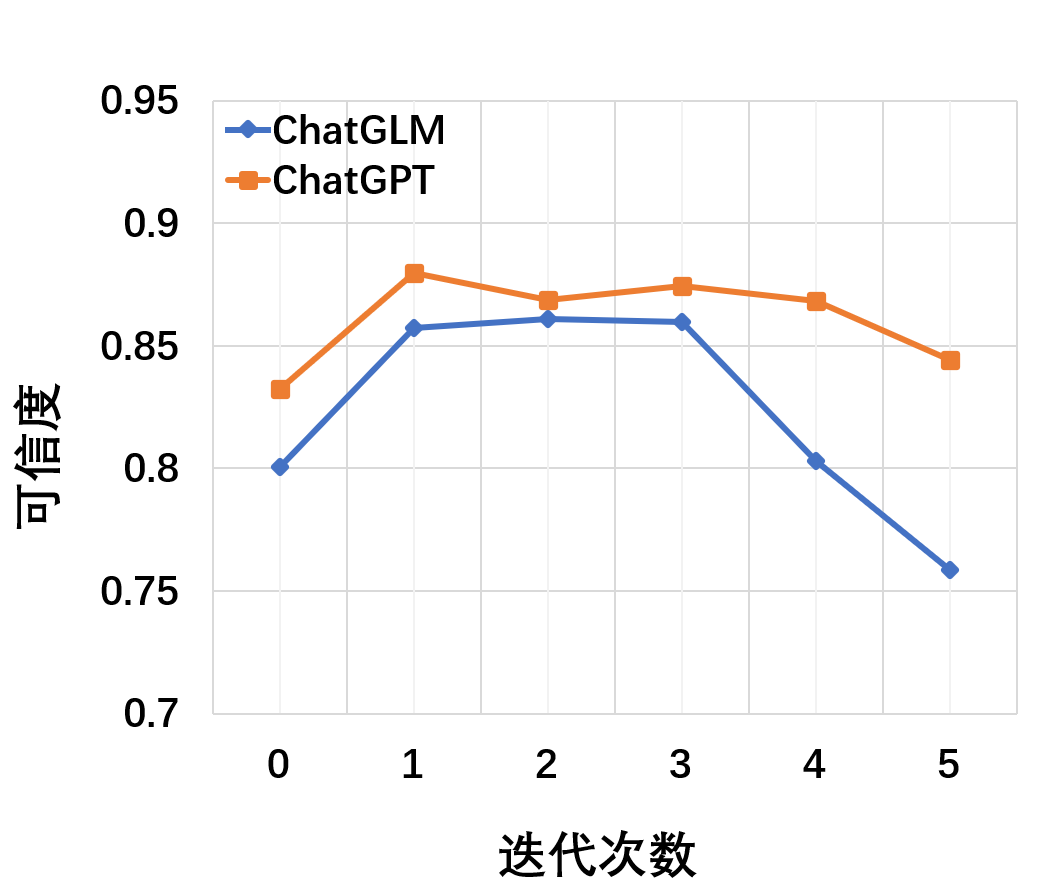
\includegraphics[width=7cm]{Fig/multi_iter_optimize_ragas_faithfulness.png}
		\caption{\label{multi_iter_optimize_ragas_faithfulness}不同迭代优化次数对可信度的影响。}
	\end{minipage}
	\begin{minipage}[t]{0.49\textwidth}
		\centering
		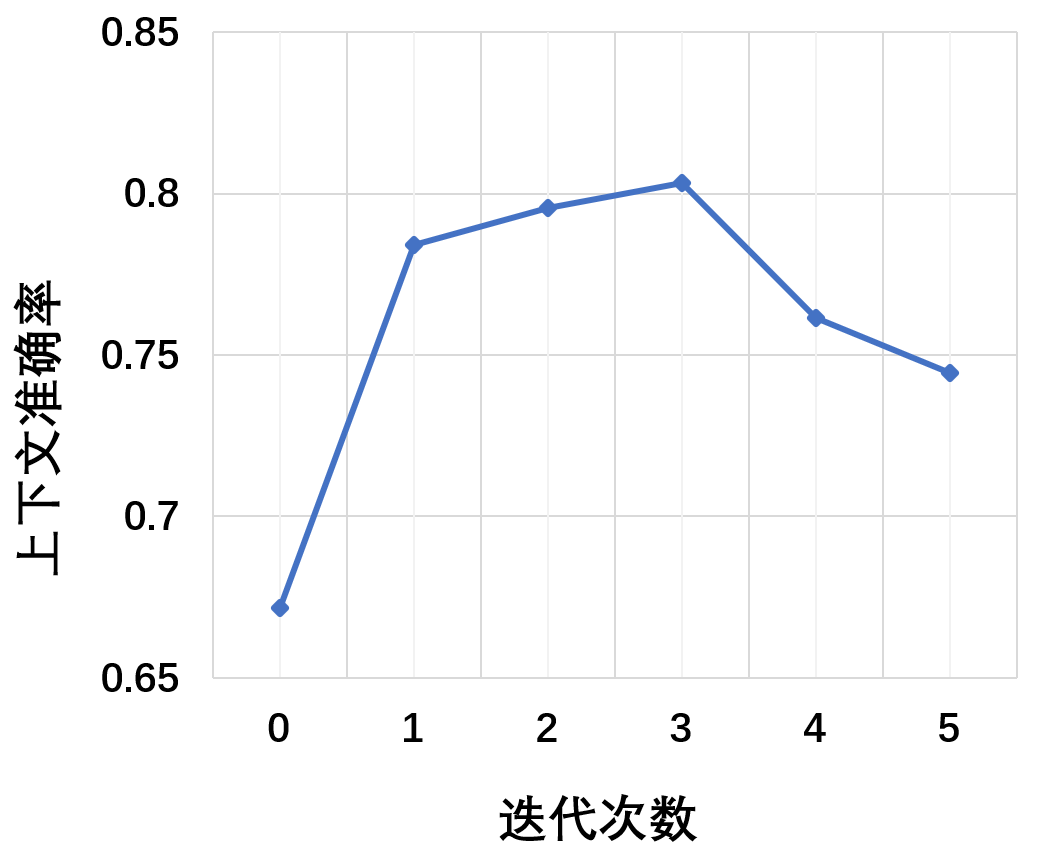
\includegraphics[width=7cm]{Fig/multi_iter_optimize_ragas_precision.png}
		\caption{\label{multi_iter_optimize_ragas_precision}不同迭代优化次数对上下文准确率的影响。}
	\end{minipage}
\end{figure}

由于QAHF可以优化用户问题以获得更好的模型回复,自然的想法是,是否可以多次迭代优化用户问题,逐步增强LLM的输出。因此,本节在AlphaFin-test数据集上进行了实验,探究迭代优化对方法性能的影响。具体来说,本节对原始用户问题进行了5次迭代优化,并与原始问题进行了Ragas可信度和上下文准确率指标的比较。如图\ref{multi_iter_optimize_ragas_faithfulness}所示,在第1次迭代中,ChatGLM和ChatGPT模型的回复可信度均有明显的改善。在前3次迭代中,可信度基本持平。而在第4次迭代时,ChatGPT性能略有下降,ChatGLM则显著降低。此外,本节还发现QAHF表现出良好的保留性,当输入的原始问题已经足够好时,QAHF有很高的概率保留它。本节认为这是实现迭代增强的关键因素,因为它避免了对用户的原始意图进行不合理的更改。

同时,本节探究迭代优化对上下文准确率指标的影响情况,即探究其对数据库知识文档检索精度的影响,结果如图\ref{multi_iter_optimize_ragas_precision}所示。在经过第1次迭代优化后,上下文准确率由0.6717显著提升至0.7839。在第2、3次优化后,准确率增速减缓,提升至0.8032。在第4、5次优化后,准确率下降到0.7444。可以看出,多次迭代优化对知识文档检索准确度的收益不高,在第4次优化后出现负面影响。

\subsection{问题有效性验证模块的有效性}

\begin{table}
	\caption{\label{evaluation_pk_fiqa}在FinGPT-FiQA数据集上探究问题有效性验证模块对性能的影响。}
	\centering
	\begin{tabular}{lcc|ccc|c}
		\toprule[2pt]
		\multirow{2}*{模型} & \multicolumn{2}{c|}{方法} & \multicolumn{3}{c|}{FinGPT-FiQA Eval} & \multirow{2}*{$\Delta$ WR} \\
		\cline{2-6}
		~ & A & B & A win & Tie & B win & ~ \\
		\hline
		\multirow{3}*{ChatGLM} & QAHF & ori. & \textbf{58.0\%} & 21.0\% & 21.0\% & +32.1\% \\
		~ & w/o Eval & ori. & \textbf{49.8\%} & 25.5\% & 24.7\% & +24.8\% \\
		~ & QAHF & w/o Eval & \textbf{8.6\%} & 86.3\% & 5.1\% & +4.5\% \\
		\bottomrule[2pt]
	\end{tabular}
\end{table}


\begin{table}
	\caption{\label{evaluation_pk_alphafin}在AlphaFin-test数据集上探究问题有效性验证模块对性能的影响。}
	\centering
	\begin{tabular}{lcc|ccc|c}
		\toprule[2pt]
		\multirow{2}*{模型} & \multicolumn{2}{c|}{方法} & \multicolumn{3}{c|}{AlphaFin-test} & \multirow{2}*{$\Delta$ WR} \\
		\cline{2-6}
		~ & A & B & A win & Tie & B win & ~ \\
		\hline
		\multirow{3}*{ChatGLM} & QAHF & ori. & \textbf{61.0\%} & 5.2\% & 33.8\% & +32.1\% \\
		~ & w/o Eval & ori. & \textbf{46.9\%} & 30.6\% & 22.5\% & +24.8\% \\
		~ & QAHF & w/o Eval & \textbf{15.1\%} & 75.3\% & 9.6\% & +4.5\% \\
		\bottomrule[2pt]
	\end{tabular}
\end{table}

QAHF的一个重要组成部分是利用反馈来优化用户指令。为了研究反馈对QAHF的快速优化有多大贡献,进行了消融实验,以比较反馈学习优化(QAHF)和直接使用ChatGPT进行快速优化。如表\ref{evaluation_pk_fiqa}和表\ref{evaluation_pk_alphafin}所示,直接优化可以提高模型性能,这验证了LLM成为良好提示工程师的潜力。QAHF提供了超越直接优化的进一步改进。这表明,纳入反馈允许LLM根据所展示的用户偏好来完善提示,从而实现更有效的提示优化。

\begin{table}
	\caption{\label{evaluation_ragas}在Ragas指标上问题有效性验证模块对性能的影响。}
	\centering
	\begin{tabular}{c|cccc}
		\toprule[2pt]
		模型 & 方法 & Precision $\uparrow$ & Recall $\uparrow$ & Faithfulness $\uparrow$ \\
		\hline
		\multirow{3}*{ChatGLM} & ori. & 0.6717 & 0.8430 & 0.8005 \\
		~ & w/o Eval & 0.7023(+0.03) & 0.8329(-0.01) & 0.8216(+0.02) \\
		~ & QAHF & 0.7839(+0.11) & 0.8417(-0.001) & 0.8574(+0.06) \\
		\bottomrule[2pt]
	\end{tabular}
\end{table}

\begin{table}
	\caption{\label{valid_invalid_example}有效样本与无效样本对比。}
	\centering
	\begin{tabular}{c|c|c}
		\toprule[2pt]
		\multicolumn{2}{c|}{类型} & 内容 \\
		\hline
		\multirowcell{3}{有效\\样本} & 原始问题 & \begin{tabular}{p{11.7cm}}
			国庆黄金周对旅游股有什么影响
		\end{tabular} \\
		\cline{2-3}
		~ & 优化问题 & \begin{tabular}{p{11.7cm}}
			国庆黄金周对旅游股有什么影响,列点回答,从宏观到微观依次分析对旅游行业、旅游公司、旅游股的影响,最后给出综合性结论。
		\end{tabular} \\
		\cline{2-3}
		~ & 模型回复 & \begin{tabular}{p{11.7cm}}
			国庆黄金周对旅游股的影响主要体现在以下几个方面:\\1.客流量增加:…\\2.板块内部分红机会:…\\3.旅游股的业绩弹性:…\\4.旅游股面临了一定的市场风险:…\\综上所述,国庆黄金周对旅游股的影响主要体现在客流量增加、板块内部分红机会、旅游股的业绩弹性和面临的市场风险等方面。投资者在关注国庆黄金周带来的投资机会的同时,还需注意国庆期间的市场风险,合理制定投资策略。
		\end{tabular} \\
		\hline
		\multirowcell{3}{无效\\样本} & 原始问题 & \begin{tabular}{p{11.7cm}}
			杭州亚运会对杭州公司股票有什么积极作用
		\end{tabular} \\
		\cline{2-3}
		~ & 优化问题 & \begin{tabular}{p{11.7cm}}
			杭州亚运会对杭州的公司有什么积极作用
		\end{tabular} \\
		\cline{2-3}
		~ & 模型回复 & \begin{tabular}{p{11.7cm}}
			杭州亚运会将为杭州的公司带来积极影响,具体来说:\\1.亚运会将带来大量游客:…\\2.亚运会将带动周边房价上涨:…\\3.亚运会将推动杭州文化产业发展:…\\4.亚运会将带动杭州基础设施建设:…\\总之,杭州亚运会将为杭州的公司带来诸多积极影响,包括游客、房价、文化产业和基础设施等方面。这些都将为杭州的公司提供更多的商业机会和发展动力。
		\end{tabular} \\
		\bottomrule[2pt]
	\end{tabular}
\end{table}

本节基于Ragas评估框架对完整的QAHF方法和去除提示词有效性验证模块后的QAHF方法进行性能比较,实验结果如表\ref{evaluation_ragas}所示。从表中结果可以看出,去除提示词有效性验证模块后,数据中噪声偏多,因此模型在Context Precision和Faithfulness指标上都仅有0.03和0.02的微弱提升,甚至在Context Recall上有0.01的降低。而增加提示词有效性验证模块后,模型在Context Precision和Faithfulness指标上有了显著提升,分别提升了0.11和0.06分,而在Context Recall指标上,与原始结果几乎相同,仅相差0.001。对于Context Recall指标上分数的降低,可能是因为问题改写仅影响模型回复与用户问题之间的相关性,而Context Recall评估的是用户问题和知识文档之间的相似性,因此在这一指标上,所对比的三种方法得分相近。

同时,表\ref{valid_invalid_example}展示了具体的有效样本和无效样本内容,从示例内容可以看出,无效样本的优化问题将原始问题中的“杭州公司股票”改为了“杭州的公司”,导致问题对象发生变化,导致最终模型回复不符合用户初始意图。有效性验证模块能够准确地从初始数据集中过滤无效样本,提高训练数据集的信噪比,避免进一步加重模型的幻觉现象。

\section{本章小结}

本章提出基于人类偏好对齐的检索增强对话生成方法,能够实现与模型无关的、可解释、效果稳定的人类偏好对齐。此外,本章提出的人类偏好对齐方法还面临着受限于标注者的主观偏好的问题,因此在未来的工作中,这也是需要进一步研究和完善的方向。